% https://mavlink.io/en/
MAVROS is an open\hyp{}source translation layer between \acs{ros} and \acs{mavlink}. \acs{mavlink} is a lightweight messaging protocol for communicating with unmanned vehicles. The key features of \acs{mavlink} are its efficiency, reliability, support of many programming languages, capability up to 255 concurrent systems on the network, and its ability to enable offboard and onboard communications. \acs{mavlink} 1 has just eight bytes overhead per packet and \acs{mavlink} 2 has fourteen to increase its security. Therefore this protocol is very well suited for applications with very limited communication bandwidth. \cite{mavlink_developer_guide}

% https://mavlink.io/en/guide/serialization.html
In this project, MAVROS is used for the communication between the written code and the \acs{uav}. MAVROS allows for coding on a higher abstraction, with the use of its library.

\begin{figure}[!h]
  \centering
  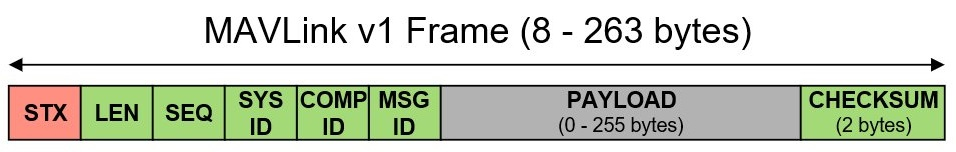
\includegraphics[width=0.65\linewidth]{images/packet_mavlink_v1.jpg}
  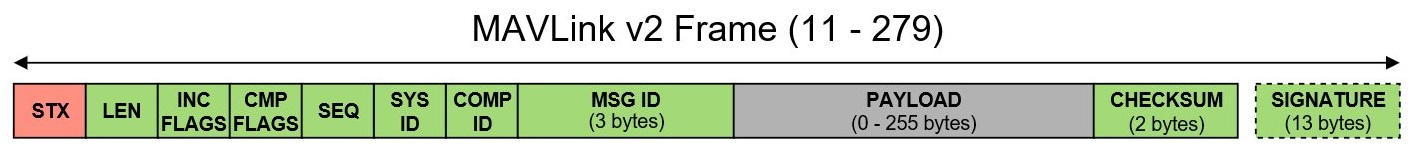
\includegraphics[width=\linewidth]{images/packet_mavlink_v2.jpg}
  \caption{MAVLink packet}
\end{figure}

\begin{table}[!h]
  \centering
  \begin{tabular}{ | >{\centering\arraybackslash}m{0.16\linewidth} | >{\centering\arraybackslash}m{0.78\linewidth} | }
    \hline
    \textbf{Name} & \textbf{Explanation} \\
    \hline
    \acs{stx} & Protocol\hyp{}specific \ac{stx} marker used to indicate the beginning of a new packet. \\
    \hline
    LEN & Indicates length of the following payload section. \\
    \hline
    INC FLAGS & Flags that must be understood for \acs{mavlink} compatibility. \\
    \hline
    CMP FLAGS & Flags that can be ignored if not understood. \\
    \hline
    SEQ & Used to detect packet loss. Increments value for each message sent. \\
    \hline
    SYS ID & ID of system (vehicle) sending the message. Used to differentiate systems on network. \\
    \hline
    COMP ID & ID of component sending the message. Used to differentiate components in a system (e.g. autopilot and a camera). \\
    \hline
    MSG ID & ID of message type in payload. Used to decode data back into a message object. \\
    \hline
    PAYLOAD & Message data. Content depends on message type (i.e. MSG ID) \\
    \hline
    CHECKSUM & X.25 \acs{crc} for the message (excluding STX byte). \\
    \hline
    SIGNATURE & (Optional) Signature to ensure the link is tamper\hyp{}proof. \\
    \hline
  \end{tabular}
  \caption{MAVLink packet explanation}
\end{table}